% !TEX root = ../report.tex

\chapter{Design}

\minitoc
This chapter the architecture and components in the architecture, how they were designed, and how they fulfill the requirements of the project.


\clearpage


\section{Definitions}


\section{Architecture}
The architecture of the project is based on The 4+1 View
Model of Software Architecture \cite{Kruchten}. The views are used reflect the structural aspects, temporal aspects, technological development aspects and physical aspects of the project.

The architecture uses a custom simplified version of the 4+1 notation that better fits the descriptive needs for the project.


\subsection{Logical View}
The logical view describes the components of the architecture and how they relate to one another in terms of containment, inheritance and usage. The logical view can be found in figure-\ref{figure:logical-view} and the notation for the logical view in figure-\ref{figure:logical-view-notation}

\begin{figure}[H]
\centerline{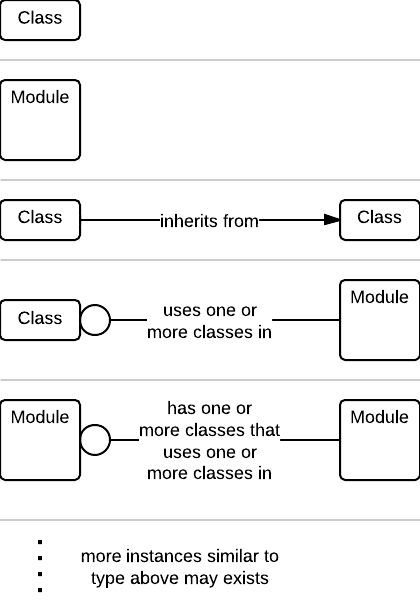
\includegraphics[width=2.5in]{image/architecture-logical-view-notation.png}}
\caption{Notation for the logical view.}
\label{figure:logical-view-notation}
\end{figure}

\begin{center}
\begin{figure}[H]
\centerline{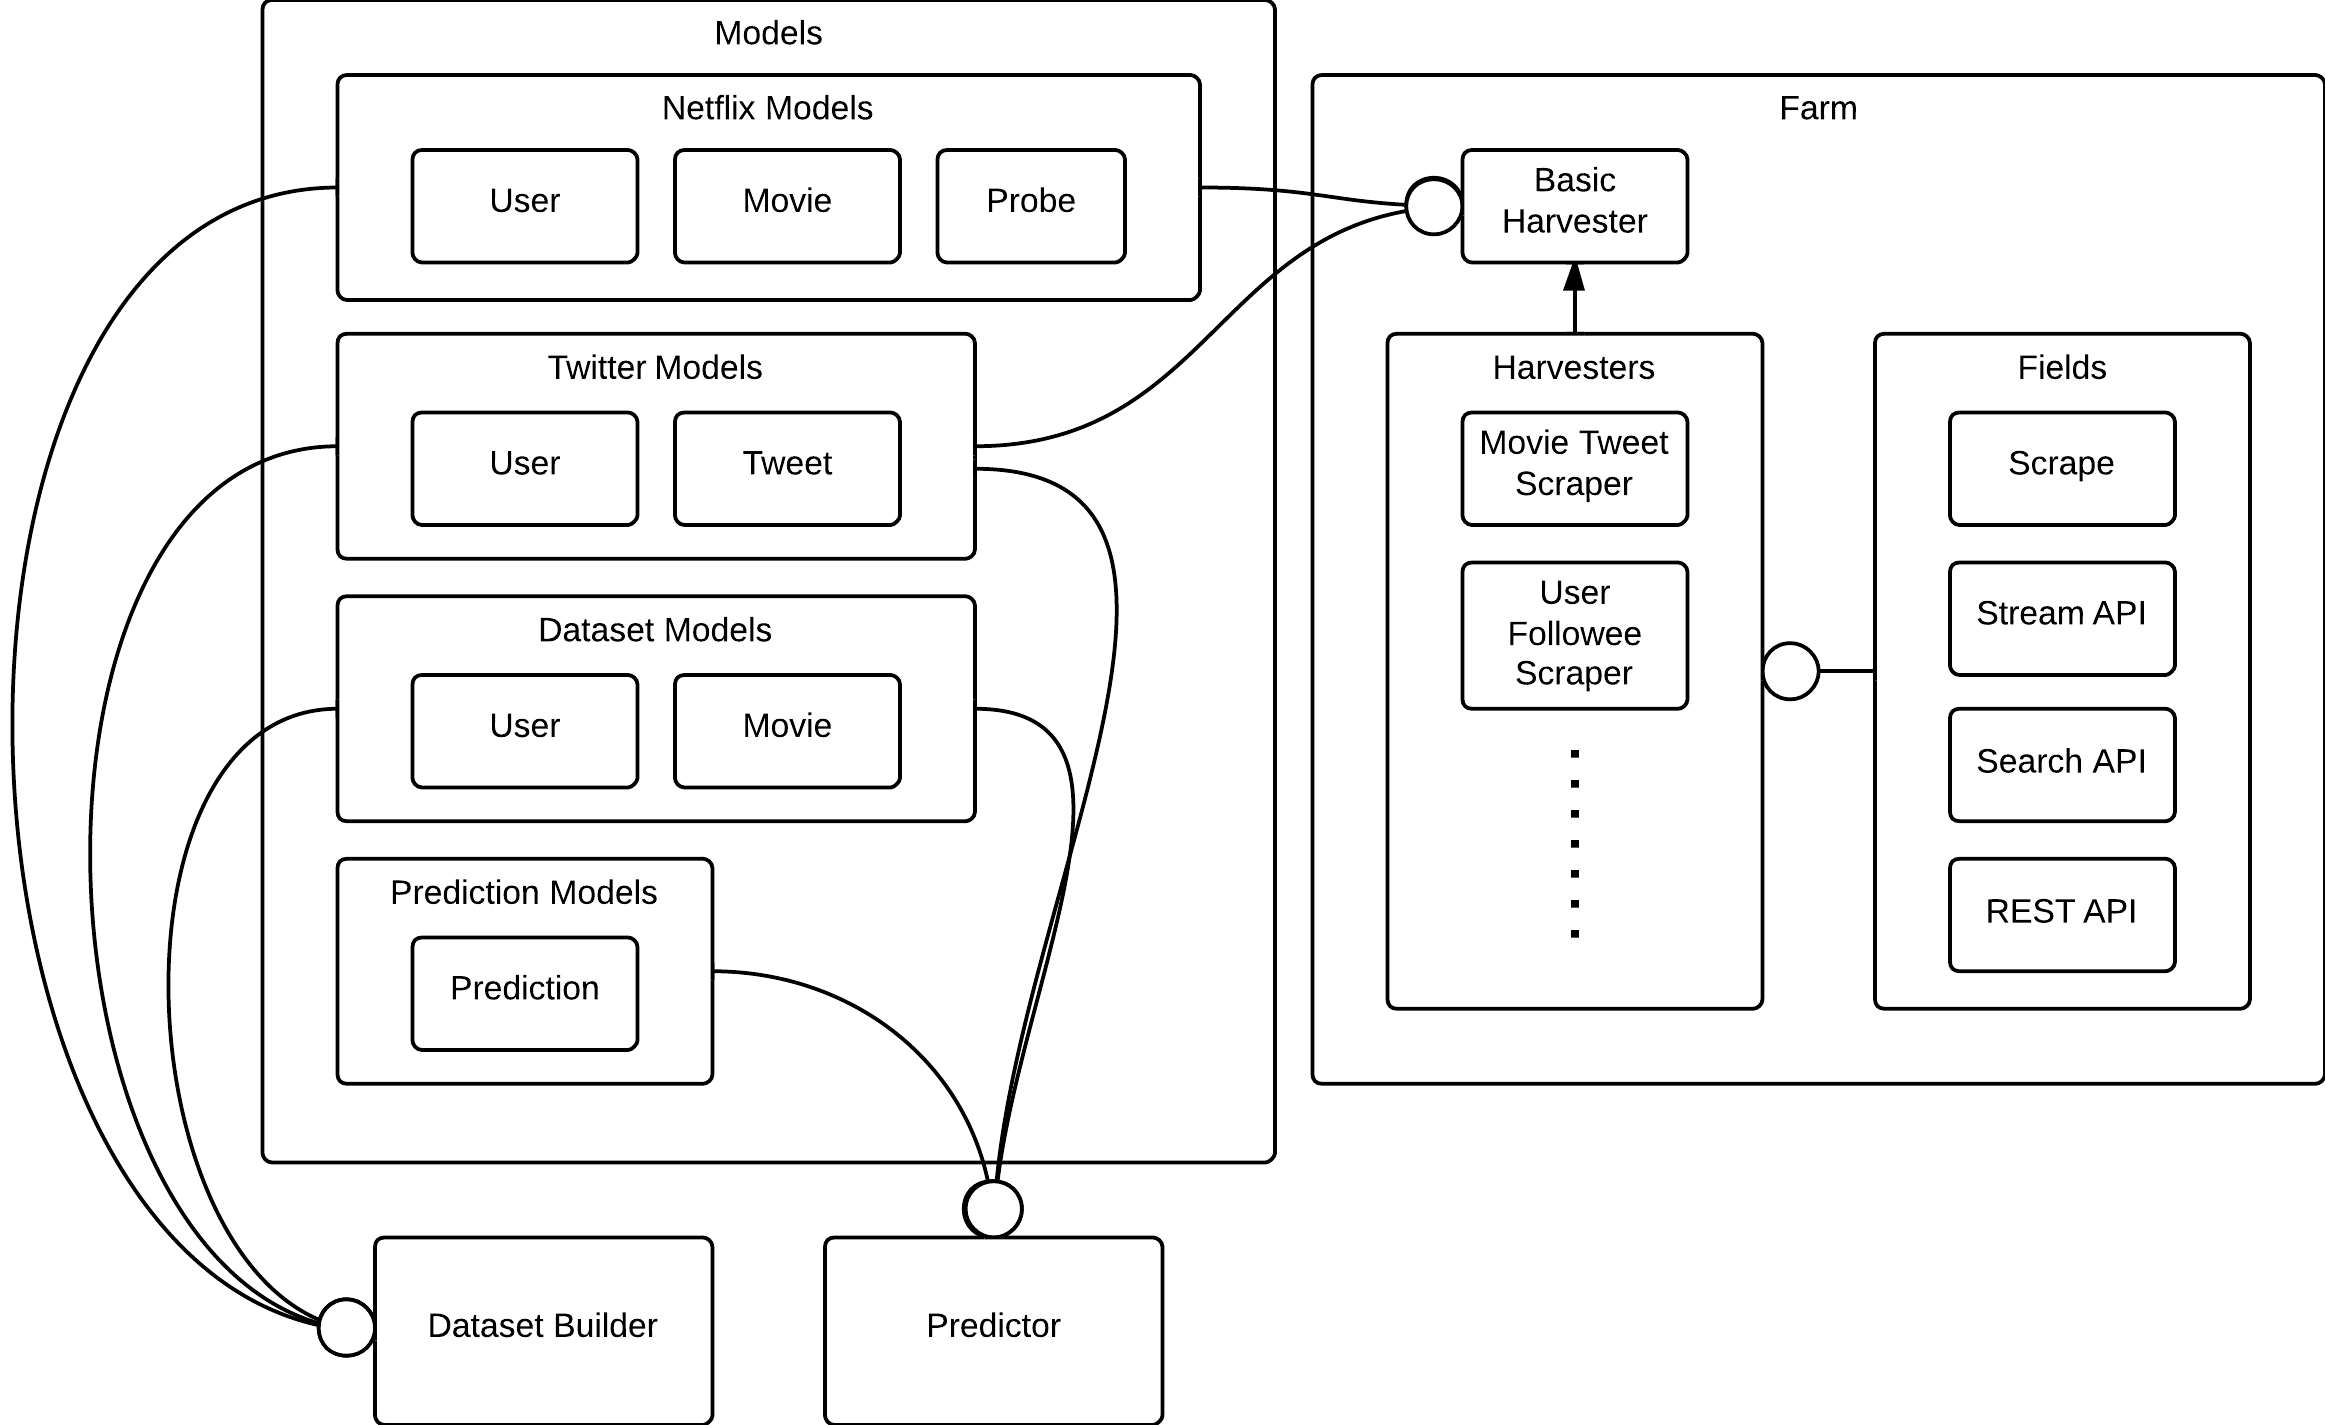
\includegraphics[width=7in]{image/architecture-logical-view.png}}
\caption{Logical view of the project. See figure-\ref{figure:logical-view-notation} for notation.}
\label{figure:logical-view}
\end{figure}
\end{center}

\subsubsection{Models}
Models is the module responsible for holding the different datamodels that are used in the project. It is found in the upper left part of the logical view in figure-\ref{figure:logical-view}. All classes in this module are mapped to and reflect the database.

The Netflix Models model the netflix prize dataset. Each user has a list of movie ratings and each movie has a list of user ratings. The probe is a list of movies with empty user ratings that need to be predicted.

The Twitter Models reflect the data harvested from Twitter. The schema of these models are variable as it depends on what type of data is harvested. A tweet typically contains a text and refers to a user. A user typically has a name and a user ID and may refer to tweets. As an example, it may also contain a list of followees or followers.

The Dataset Models reflects the Netflix Models after they have been mapped to fused with Twitter Models by the Dataset Builder.

The Prediction Models model what the ratings that the Predictor predicts using the Datast Models and the Probe in Netflix Models.

\subsubsection{Farm}


\subsubsection{Dataset Builder}

\subsubsection{Predictor}


\subsection{Process View}
The process view describes the actions that the components of the architecture engage in over time and how there actions relate to other components.

\subsection{Development View}
describes the mapping(s) of the software onto the hardware. reflects hardware distribution if present

\begin{figure}[H]
\centerline{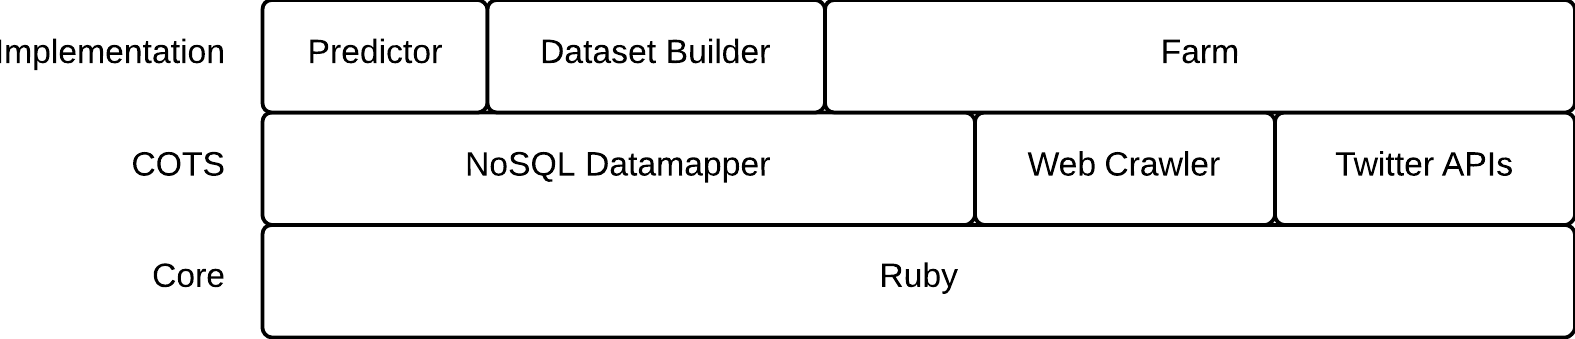
\includegraphics[width=4.5in]{image/architecture-development-view.png}}
\caption{Development view showing the technology stack. Each technology block is dependent on the technology block(s) below it.}
\label{figure:development-view-notation}
\end{figure}

\subsection{Physical View}
describes the mapping(s) of the software onto the hardware. reflects hardware distribution if present

\subsection{Scenarios}

\section{Component Design}


